\begin{table}[H]
    \centering
	\begin{tabular}{lcccc}
	\textbf{Layer Type} & \textbf{Layer Config} & \textbf{Activation}  & \textbf{Output} & \textbf{Params}\\ \hline
	\conv	& \convKSF{5}{3}{5}	& relu		& \texttt{48,86,5} 	& \texttt{380}\\
	\conv	& \convKSF{5}{2}{8}	& relu		& \texttt{24,43,8} 	& \texttt{1008}\\	
	\conv	& \convKSF{3}{1}{12}	& relu		& \texttt{24,43,12} 	& \texttt{876}\\
	\conv	& \convKSF{3}{1}{15}	& relu		& \texttt{24,43,15} 	& \texttt{1635}\\
	\conv	& \convKSF{3}{1}{18}	& relu		& \texttt{24,43,18} 	& \texttt{2448}\\
	
	\flt		& /					& /		& \texttt{20640}		& \texttt{0}\\
	\dns		& \dnsP{64}			& relu		& \texttt{64}		& \texttt{1188928}\\
	\dns		& \dnsP{6}			& softmax	& \texttt{6}		& \texttt{390}\\
	\multicolumn{4}{r}{\textbf{TOTAL}}&{\textbf{1,195,665}}\\
	\end{tabular}
	%Total params: 1,195,665
	%Trainable params: 1,195,665
	%Non-trainable params: 0
\end{table}


\begin{table}[H]
	\centering
	\begin{tabular}{lc}
	\textbf{Param} & \textbf{Value}\\ \hline
	Batch Size 	& 32 \\
	Optimizer 	& Adam \\
	Base lr		& 0.001 \\
	Epochs		& 20 \\
	\end{tabular}
\end{table}


\begin{figure}[H]
	\begin{center}
	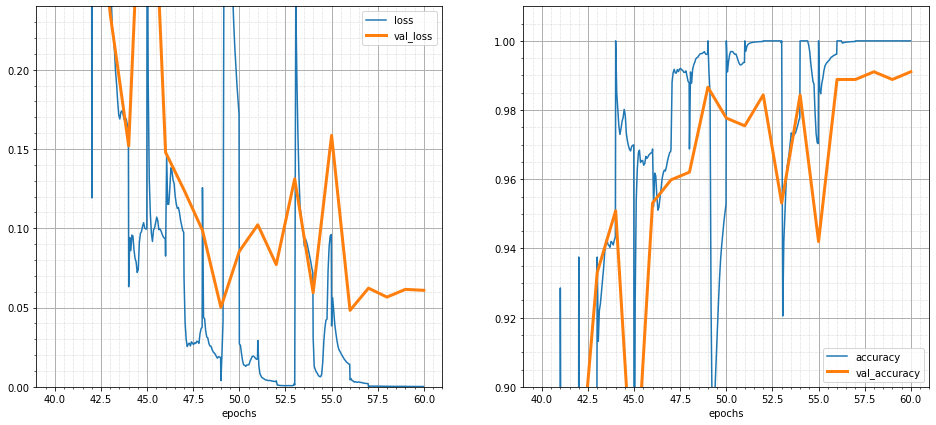
\includegraphics[width=\linewidth]{Immagini/conv-3}
	\caption{Graph of the third run}
	\end{center}
\end{figure}
\begin{table}[H]
	\centering
	\begin{tabular}{cccccc}
		\textbf{Run} &\textbf{Loss}&\textbf{V.Loss} &\textbf{Acc.}&\textbf{V.Acc.}&\textbf{$\Delta$ Acc.} \\ \hline
		1   & 1.0908e-04    &   0.0439  & 1.0000    & 0.9866    & 0.0134 \\
		2   & 8.7761e-05    &   0.0912  & 1.0000    & 0.9888    & 0.0112 \\
		3   & 1.8083e-04    &   0.0609  & 1.0000    & 0.9911    & 0.0089 \\
		\textbf{Avg} & \textbf{1.2589e-04} & \textbf{0.0653}	& \textbf{1.0000}	& \textbf{0.9889} 	& \textbf{0.0112} 
	\end{tabular}
\end{table}

This models is an iteration of the baseline model, achieved by adding four more convolution. The convolution have been added with the following logic in mind:
\begin{itemize}
\item The first two convolutions have a stride greater than 1, and that leads to a minimal reductions in the size of the tensor. This in turn should limit the number of parameters needed for training and in turn reduce overfitting.
\item The layers are set in way to progressively increase the number of channel and reduce height and width.
\end{itemize}
The results show the model is slightly less overfitting than the baseline. Both models reached 1.0000 accuracy on the training set, so this translate in an increased validation accuracy.
%NOTARE CHE AGGIUNGERE PIU LIVELLI NON AIUTA



